\documentclass[tikz]{standalone}
\usepackage{pgfplots}
\usepgfplotslibrary{groupplots}
\pgfplotsset{width=8.4cm, height=7cm, compat=1.18}
\usepackage{tikz}
\usepackage{gensymb}
\usepackage{amsmath}

\def\myline{very thick}

\begin{document}
	% This file was created with tikzplotlib v0.10.1.
	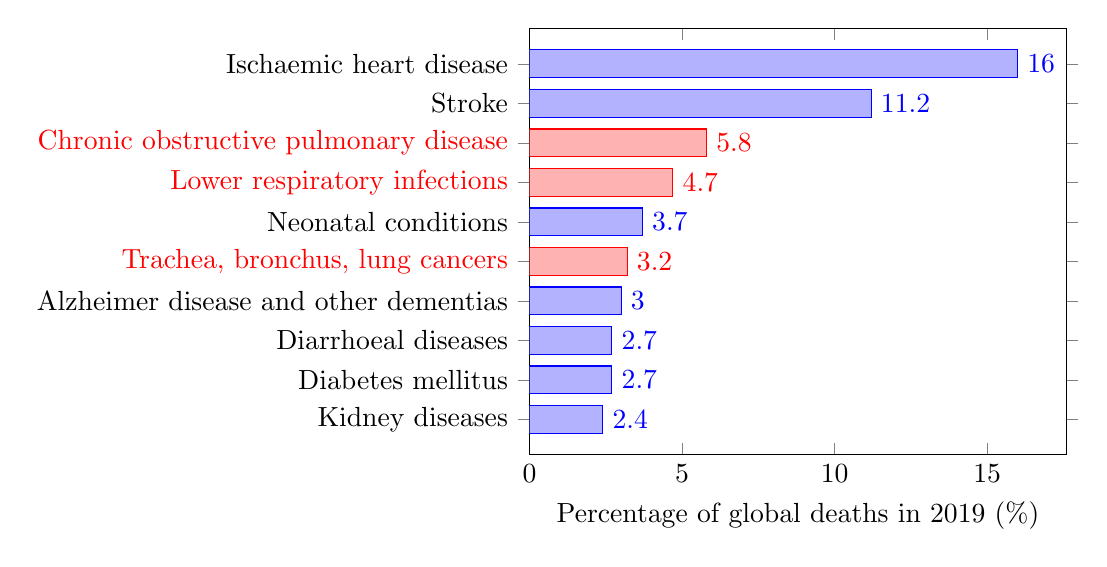
\begin{tikzpicture}
		\begin{axis}[
			xbar, xmin=0,
			xlabel={Percentage of global deaths in 2019 (\%)},
			symbolic y coords={
				{Kidney diseases},
				{Diabetes mellitus},
				{Diarrhoeal diseases},
				{Alzheimer disease and other dementias},
				{Trachea, bronchus, lung cancers},
				{Neonatal conditions},
				{Lower respiratory infections},
				{Chronic obstructive pulmonary disease},
				{Stroke},
				{Ischaemic heart disease}
			},
			ytick distance=1,
			ytick={
				{Kidney diseases},
				{Diabetes mellitus},
				{Diarrhoeal diseases},
				{Alzheimer disease and other dementias},
				{Trachea, bronchus, lung cancers},
				{Neonatal conditions},
				{Lower respiratory infections},
				{Chronic obstructive pulmonary disease},
				{Stroke},
				{Ischaemic heart disease}
			},
			yticklabels={
				{Kidney diseases},
				{Diabetes mellitus},
				{Diarrhoeal diseases},
				{Alzheimer disease and other dementias},
				\textcolor{red}{Trachea, bronchus, lung cancers},
				{Neonatal conditions},
				\textcolor{red}{Lower respiratory infections},
				\textcolor{red}{Chronic obstructive pulmonary disease},
				{Stroke},
				{Ischaemic heart disease}
			},
			nodes near coords, 
			nodes near coords align={horizontal},
			/pgf/bar shift={0pt},
			]
			\addplot coordinates {
				(16.0,{Ischaemic heart disease})
				(11.2,{Stroke})
				(3.7,{Neonatal conditions})
				(3.0,{Alzheimer disease and other dementias})
				(2.7,{Diarrhoeal diseases})
				(2.7,{Diabetes mellitus})
				(2.4,{Kidney diseases})
			};
			\addplot coordinates {
				(5.8,{Chronic obstructive pulmonary disease})
				(4.7,{Lower respiratory infections})
				(3.2,{Trachea, bronchus, lung cancers})
			};
		\end{axis}
	\end{tikzpicture}
\end{document}
